%%%%%%%%%%%%%%%%%%%%%%%%%%%%%%%%%%%%%%%%%
% Structured General Purpose Assignment
% LaTeX Template
%
% This template has been downloaded from:
% http://www.latextemplates.com
%
% Original author:
% Ted Pavlic (http://www.tedpavlic.com)
%
% Note:
% The \lipsum[#] commands throughout this template generate dummy text
% to fill the template out. These commands should all be removed when 
% writing assignment content.
%
%%%%%%%%%%%%%%%%%%%%%%%%%%%%%%%%%%%%%%%%%

%----------------------------------------------------------------------------------------
%	PACKAGES AND OTHER DOCUMENT CONFIGURATIONS
%----------------------------------------------------------------------------------------

\documentclass{article}

\usepackage{fancyhdr} % Required for custom headers
\usepackage{lastpage} % Required to determine the last page for the footer
\usepackage{extramarks} % Required for headers and footers
\usepackage{graphicx} % Required to insert images
\usepackage{lipsum} % Used for inserting dummy 'Lorem ipsum' text into the template
\usepackage{authblk}
\usepackage{amsmath, amssymb}
\usepackage{hyperref}
\usepackage{booktabs,multirow}
\usepackage{xcolor}
\usepackage{listings}
\usepackage{textcomp}
\usepackage{setspace}
\usepackage{palatino}

\graphicspath{{imgs/}}

\renewcommand{\lstlistlistingname}{Code Listings}
\renewcommand{\lstlistingname}{Code Listing}
\definecolor{gray}{gray}{0.5}
\definecolor{green}{rgb}{0,0.5,0}

\lstnewenvironment{python}[1][]{
\lstset{
language=python,
numbers=left, numberstyle=\tiny,
basicstyle=\ttfamily\small\setstretch{1},
stringstyle=\color{red},
showstringspaces=false,
alsoletter={1234567890},
otherkeywords={\ , \}, \{},
keywordstyle=\color{blue},
emph={access,and,break,class,continue,def,del,elif ,else,%
except,exec,finally,for,from,global,if,import,in,i s,%
lambda,not,or,pass,print,raise,return,try,while},
emphstyle=\color{orange}\bfseries,
emph={[2]True, False, None, self},
emphstyle=[2]\color{green},
emph={[3]from, import, as},
emphstyle=[3]\color{blue},
upquote=true,
morecomment=[s]{"""}{"""},
commentstyle=\color{gray}\slshape,
emph={[4]1, 2, 3, 4, 5, 6, 7, 8, 9, 0},
emphstyle=[4]\color{blue},
literate=*{:}{{\textcolor{blue}:}}{1}%
{=}{{\textcolor{blue}=}}{1}%
{-}{{\textcolor{blue}-}}{1}%
{+}{{\textcolor{blue}+}}{1}%
{*}{{\textcolor{blue}*}}{1}%
{!}{{\textcolor{blue}!}}{1}%
{(}{{\textcolor{blue}(}}{1}%
{)}{{\textcolor{blue})}}{1}%
{[}{{\textcolor{blue}[}}{1}%
{]}{{\textcolor{blue}]}}{1}%
{<}{{\textcolor{blue}<}}{1}%
{>}{{\textcolor{blue}>}}{1},%
framexleftmargin=1mm, framextopmargin=1mm, frame=shadowbox, rulesepcolor=\color{blue},#1
}}{}

% Margins
\topmargin=-0.45in
\evensidemargin=0in
\oddsidemargin=0in
\textwidth=6.5in
\textheight=9.0in
\headsep=0.25in 

\linespread{1.1} % Line spacing

% Set up the header and footer
\pagestyle{fancy}
\lhead{\hmwkAuthorName} % Top left header
\chead{\hmwkClassID\ (\hmwkClassInstructor\ - \hmwkClassTime)} % Top center header
\rhead{\hmwkTitle} % Top right header
\lfoot{\lastxmark} % Bottom left footer
\cfoot{} % Bottom center footer
\rfoot{Page\ \thepage\ of\ \pageref{LastPage}} % Bottom right footer
\renewcommand\headrulewidth{0.4pt} % Size of the header rule
\renewcommand\footrulewidth{0.4pt} % Size of the footer rule

\setlength\parindent{0pt} % Removes all indentation from paragraphs


   
%----------------------------------------------------------------------------------------
%	NAME AND CLASS SECTION
%----------------------------------------------------------------------------------------

\newcommand{\hmwkTitle}{Project Report} % Assignment title
\newcommand{\hmwkDueDate}{Thursday,\ October\ 16,\ 2014} % Due date
\newcommand{\hmwkClassID}{CS5330} % Course/class
\newcommand{\hmwkClassName}{Randomized Algorithm} % Course/class
\newcommand{\hmwkClassTime}{Thu, 06:30pm} % Class/lecture time
\newcommand{\hmwkClassInstructor}{Dr. Lee Hwee Kuan} % Teacher/lecturer
\newcommand{\hmwkAuthorName}{LIU Weizhi} % Your name
\newcommand{\hmwkAuthorEmail}{weizhiliu2009@gmail.com} % Your email

%----------------------------------------------------------------------------------------
%	TITLE PAGE
%----------------------------------------------------------------------------------------

\title{
\vspace{2in}
\textmd{\textbf{\hmwkClassID \ - \hmwkClassName }}\\
\textmd{\textbf{\hmwkTitle}}\\
\normalsize\vspace{0.1in}\small{Due\ on\ \hmwkDueDate}\\
\vspace{0.1in}\large{\textit{\hmwkClassInstructor\ - \hmwkClassTime}}
\vspace{3in}
}

\author{\textbf{\hmwkAuthorName} \thanks{\hmwkAuthorEmail}}
\affil{Department of Industrial \& Systems Engineering \\ National University of Singapore}
\date{\today} % Insert date here if you want it to appear below your name

%----------------------------------------------------------------------------------------

\begin{document}

\maketitle

%----------------------------------------------------------------------------------------
%	TABLE OF CONTENTS
%----------------------------------------------------------------------------------------

%\setcounter{tocdepth}{1} % Uncomment this line if you don't want subsections listed in the ToC

% \newpage
% \tableofcontents
% \newpage

\newpage

\begin{center}
\textbf{\large{Maximizing Network Reward Based on A Genearal Framework \\ of Monte Carlo Tree Search }}
\end{center}

\begin{abstract}
This study implemented the general framework of MCTS to solve the network population problem. Preliminary comparision of different algorithms demonstrates that uct0.5 and uct1.0 perform best in both criteria of best rewards detection and computation time, especially, uct seems like possessing the abality of learning. While rmc and nmc1 performs much faster than the other algorithms, their abality of detecting best population sequence is poor. An interesting finding is that there might exist some periods for nmc2 algorithms in terms of reward sequence.\\

\textbf{Keywords: Monte Carlo Tree Search, Multi-armed Bandit Problem, Network Population}
\end{abstract}

\section{Introduction}
The goal of the project is to search the optimal network population sequence in order to maximize the total reward of the network given two input files, namely an undirected network adjacent list and original color sequence. The network adjacent list file depicts which node connects to the other node, and the network may contain self-loop and multiple edges. The original color sequence is a 0/1 binary sequence, which illustrates the order of the color sequence (eg. 0 represents red, 1 represents blue). The total reward of the network is calculated by summing up all the numbers of edges which connect to two different color nodes (note that we only consider colored node, and the uncolored nodes have no color at all). At the initial stage of the game, one should pick an arbitrary node from the network and color it according to the corresponding color from the original color sequence. Then the next population candidate could only be selected from those nodes which are not colored yet and connect to at least one already colored node. The game will enter into termial state when the original color sequence runs out or there are no further possible candidate nodes to color. All in all, the aim of this game is to select an optimal enough population sequence to maximize the total reward of the network.\\

Obviously, when the graph is large enough, the naive brute force algorithm could consume enormous time which is not acceptable given a limited computation budget. One possible and efficient way to solve this game is to implement Monte Carlo Tree Search (MCTS) algorithms which have gained remarkable attentations in the past few years, especially after the significant success on the game of Go \cite{coulom2007efficient}. However, there are various MCTS algorithms (eg. UCT \cite{kocsis2006bandit}, Nested Monte Carlo (NMC) search \cite{cazenave2009nested}, Reflexive Monte Carlo (RMC) search \cite{cazenave2007reflexive}) for which may only perform well on some certain problems. Therefore, for a specificed problem, a domain based algorithm will be designed to best fit that problem. However, it's very difficult to design a domain based algorithm which needs more deep understanding of the original problem. To facilitate this process, this paper implemented a more general framework of MCTS which can generate all possible popular MCTS algorithms nowadays based on the work of Francis Maes et al. (\cite{maes2012monte}). The remainder of this paper are as follows. The general framework of MCTS is proposed in section 2, followed by the comparision results and current network best rewards for different sets in section 3. Finally, we conclude this paper by summarizing the important facts and possible future work.

\section{Method}
The important notations of this paper is listed in Table \ref{tab:notations}. In this section, the network construction and reward evaluation is illustrated firstly and then the general framework of MCIS will be discussed.

\begin{table}[htbp]
  \centering
  \caption{Notations}
    \begin{tabular}{cc}
    \toprule
    notation &  definition \\
    \midrule
    $\mathcal{A}_{n \times n}$ & adjacent matrix of the network with $n$ nodes\\
    $a_{ij}$ & element of $\mathcal{A}_{n \times n}$ which represents the number of edges between node $i$ and $j$ \\
    $\vec s$ & the original input sequence \\
    $\vec c_{1 \times n}$ & color vector for every nodes, $c_{i}$ represents the color of node $i$\\
    $r_{ij}$ & reward value between node $i$ and node $j$\\
    $R(\mathcal{A}_{n \times n}, \vec c_{1 \times n})$ & total reward of the network \\
    $R^{*}$ & current best network reward \\
    $w_{k}$ & the candidate nodes set at step $k$\\
    $\vec p_{k} = (p_{1}, p_{2}, \cdots, p_{k})$ & population sequence at step $k$ of which element $p_{i}$ represents the $i$th populated nodes\\
    $\vec p^{*}$ & current best population sequence \\
    $\tau(k)$ & represents if the game enters into end at time $k$\\
    $B$ & total budget for each algorithm \\
    $numCalls$ & current times of evaluation \\
    $\mathcal{S}$ & search component \\
    $N^{(repeat)}$ & repeat times for repeat component \\
    $N^{(select)}$ & multiple factor for select component \\
    $\eta$ & weight factor for exploring of ucb value \\
    $\mathcal{L}_{i}$ & the lower level search component standalone parameters recursive list at level $i$\\
    \bottomrule
    \end{tabular}%
  \label{tab:notations}%
\end{table}%

\subsection{Network Construction and Reward Evaluation}
The network $\mathcal{A}_{n \times n}$ could be constructed based on the network adjacent list by continuously update $a_{ij}$. Since the network is undirected, $a_{ij}$ should be the same with $a_{ji}$.\\

The $i$th elemet of color vector $\vec c_{1 \times n}$ equals to the following value conditioning on the color of the $i$th node
\begin{align}
  c_{i} = \left \{
             \begin{array}{cl}
               -1 & \mbox{if node $i$'s color is 0} \\
               0 & \mbox{if node $i$ is not colored} \\
               1 & \mbox{if node $i$'s color is 1} \\
             \end{array}
          \right.
\end{align}
Thus, we can easily calculate the reward between node $i$ and node $j$ given a network $A_{n \times n}$ and color vector $\vec c_{1 \times n}$ based on the equation (\ref{eq:reward})
\begin{equation}
\begin{aligned}
  \label{eq:reward}
  r_{ij} = \frac{(c_{i}c_{j} - 1)}{2} c_{i} c_{j} a_{ij} = \frac{1}{2} (c_{i}^{2}a_{ij}c_{j}^{2} - c_{i}a_{ij}c_{j})
\end{aligned}
\end{equation}
Consequently, the total reward of the network could be formulated in a matrix expression (also note that the network $\mathcal{A}_{n \times n}$ is symmetric)
\begin{equation}
\begin{aligned}
  R(\mathcal{A}_{n \times n}, \vec c_{1 \times n}) =  \frac{1}{4} [(\vec c_{1 \times n})^{2} \mathcal{A}_{n \times n} (\vec c_{1 \times n}^{T})^{2} - \vec c_{1 \times n} \mathcal{A}_{n \times n} \vec c_{1 \times n}^{T}]
\end{aligned}
\end{equation}

\subsection{General Framework of MCTS}
The general framework of MCTS in this article consists of five helper components and five search components. The detailed description of each component is presented at the following parts. In addition, an algorithm generator should be designed which could create and implement many MCTS algorithms after specifying the recursive relationships between search componets and necessary parameters.

\subsubsection{Helper Components}
Table \ref{tab:helper_components} depicts the five helper componets and their corresponding task. A more detailed implementation of this componets could be seen in the Appendix B.

\begin{table}[htbp]
  \centering
  \caption{Illustration of helper components}
    \begin{tabular}{cccc}
    \toprule
    helper component &  task  & input & output \\
    \midrule
    candidate & update candidate nodes set for populating & $\vec p_{k-1}, p_{k}, w_{k-1}$ & $w_{k}$\\
     & by set operation rather than loop& & \\
    terminal & check wheter the game enters into end & $\vec p_{k}, w_{k}$ & $\tau(k)$ \\
    reward & calculate the network reward & $\mathcal{A}_{n \times n}, \vec c_{1 \times n}$ & R\\
    evaluate & update the budget consumption, best & $\vec p_{k}, \vec p^{*}, R^{*}, \mathcal{A}_{n \times n}, \vec c_{1 \times n}$ & \\
      & reward and population sequence & $numCalls, B$ & $\vec p^{*}, R^{*}, numCalls$ \\
    invoke & invoke other search components & $\vec p_{k}, w_{k}, \mathcal{S}$ & $\vec p_{m} (m > k)$ \\
    \bottomrule
    \end{tabular}%
  \label{tab:helper_components}%
\end{table}%

\subsubsection{Search Components}
Table \ref{tab:search_components} illustrates the five search componets and their corresponding task. Note that the input of all five search components include the current population sequence $\vec p_{k}$ and next candidate node set $w_{k}$ and the output should be a best full or partial population sequence if the search components generate and evaluate many possible population sequences, or just a population which might not be best (eg. simulate component just return a uniformly randomly selected full population sequence). In addition, the repeat component should receive another parameter, namely the total repeat times $N^{(repeat)}$, while select component contains two more input parameters, namely the multiple factor $N^{(select)}$ and the weight factor $\eta$ of exploring for the ucb value. Furthermore, in order to generate more algorithms recurisively, the study has proposed two different types of search components with regard to whether it can invoke the other search component. One is \textbf{atom component} which can not invoke the other search component (eg. simulate component), and the other one is \textbf{free component} (in this framework, eg. step, repeat, lookahead, select) which can invoke the other component even themselves. Those free component, compared with the atom component, include another input parameter called \textbf{lower level search component standalone parameters recurisive list} which contains all the standalone parameters and further \textbf{lowe level search component standalone parameters recursive list} for the lower level search component. The lowe level search component represents the the set of all further invoking search components of the current search component. For example, if one algorithm is like step(repeat(select(simulate(), $N^{select}, \eta$), $N^{repeat}$)), then the lower level search component of repeat component is just select and simulate. \\

Most of search components here are same with those of Maes et al. (\cite{maes2012monte}) despite the select component. There are basically two major differences
\begin{itemize}
  \item the budget for select component is automatically adjusted according to the size of graph and sequence, and the step of current population sequence which can be formulated as below at step $k$
    \begin{align}
      Budget(k)^{select} = Size(w_{k}) [(1 - \frac{Dim(\mathcal{A}_{n \times n}) N^{select}}{Size(w_{k})}) \frac{Size(\vec p_{k})}{Size(\vec s)} + \frac{Dim(\mathcal{A}_{n \times n}) N^{select}}{Size(w_{k})}]
    \end{align}
    Actually, the initial budget is just $Dim(\mathcal{A}_{n \times n}) N^{select}$ and the last budget is only $Size(w_{k})$. Therefore, this automatic budget allocation will efficiently reduce the budget resoruces when the algorithms have explored many possible population sequences.
  \item Since the reward part and explore part of ucb value in this problem is extremely different with regard to the scale, therefore it's necessary to normalize the two parts. Reward part is divided by the current best rewatd, while the explore part is transformed into $(0,1)$ via logistic function. However, since the possible population sequence space is really large, and it might be impossible to find the best population sequence which means normalize the two parts will increase the possibliy of exploring which is not efficient. After finding that new ucb value doesn't improve the best reward, so I finally give up this approach and implement the traditional way (actually, I think the original reward part of ucb value should be scaled into $[0,1]$).
\end{itemize}


\begin{table}[htbp]
  \centering
  \caption{Illustration of search components}
    \begin{tabular}{ccc}
    \toprule
    search component &  task & type\\
    \midrule
    simulate & uniformly randomly select a full population sequence & atom component\\
    step & generate a full population sequence step by step & free component\\
    repeat & return the best population by repeating $N^{repeat}$ times evaluation & free component\\
    lookahead & return the best population by evaluating full population &  \\
    & sequence among all next candidates & free component\\
    select & a mini version of UCB & free component\\
    \bottomrule
    \end{tabular}%
  \label{tab:search_components}%
\end{table}%xs
The detailed implementation of each search component can be seen in the Appendix B.

\subsubsection{Algorithms Generator}
Based on the help of basic search component, dozens of MCTS algorithms could be defined. For example, the possible popular MCTS algorithms are listed in Table \ref{tab:algo_examples}.
\begin{table}[htbp]
  \centering
  \caption{MCTS algorithms examples based on the general framework}
    \begin{tabular}{cc}
    \toprule
    algorithm & recursive expression\\
    \midrule
    rmc($N_{1}^{select}, N_{2}^{select}$) & step(repeat($N_{1}^{select}$, step(repeat($N_{2}^{select}$, simulate()))))\\
    nmc(1) & step(lookahead(simulate())) \\
    nmc(2) & step(lookahead(step(lookahead(simulate())))) \\
    uct($N^{repeat}, N^{select}, \eta$) & step(repeat($N^{repeat}$, select($N^{select}, \eta$, simulate())))\\
    \bottomrule
    \end{tabular}%
  \label{tab:algo_examples}%
\end{table}%xs
Many other possible algorithms could be seen in Maes et al.\cite{maes2012monte}. Actually, the recursive expression could be implemented by \textbf{functional programming}. However, I have little knowledge about that, but I have figured out my way to implement the recursive expression by the \textbf{lower level search component standalone parameters recursive list} mentioned before. The implementation of the algorithms generator based on python is revealed in the next section.

\section{Results \& Discussion}

\subsection{Datasets}
There are 7 datasets and the size of network and original sequence (which will influence the population search space) are illustrated in Table \ref{tab:datasets}. Consequently, a possible simulation path should be set 1, set 2, set 3, set 6, set 4, set 5 and set 7 considering the difficulity of different datasets.

\begin{table}[htbp]
  \centering
  \caption{Descriptions of datasets}
    \begin{tabular}{ccc}
    \toprule
    dataset & network size (range) & sequence size \\
    \midrule
    set 1 & 10 & 10 \\
    set 2 & 153 & 20 \\
    set 3 & 153 & 130 \\
    set 4 & 961 & 400 \\
    set 5 & 5002 & 4000 \\
    set 6 & 483 & 400 \\
    set 7 & 11748 & 9000 \\
    \bottomrule
    \end{tabular}%
  \label{tab:datasets}%
\end{table}%

\subsection{Algorithms Comparisions}
To decide which algorithms (one or more) may be more efficient to solve this problem, five basic algorithms were evaluated in the terms of optimality and computation time based on set 2. The five algorithms include rmc(10000,10), nmc1, nmc2, uct0.5 (which means the exploring weight factor is 0.5), uct1.0. The comparision of optimality could be seen in Figure \ref{fig:optimality}, while Figure \ref{fig:computation_time} depicits the difference on computation time. For each algorithm, 10000 budget are allocated to it and 10 independently simulation runs are conducted. Apart from this, the trend of best reward against each full population evaluation is illustrated in Figure \ref{fig:trends_rmc} - \ref{fig:trends_uct1.0}. Though nmc1 is the most fast algorithms, its abality to find the optimal population sequence is not so good. While uct0.5 and uct1.0 performs best in both criterias of best rewards and computation time. In addition, note that uct0.5 and uct1.0 seems to improve their performance continuously based on Figure \ref{fig:trends_uct0.5} and Figure \ref{fig:trends_uct1.0}. Consequently, this study implement these two algorithms and then find the best population sequence from them. Another remarkable finding is that the there might exists some periods in the reward sequence of nmc2 according to Figure \ref{fig:trends_nmc2}.

\begin{figure}[htbp!]
\centering
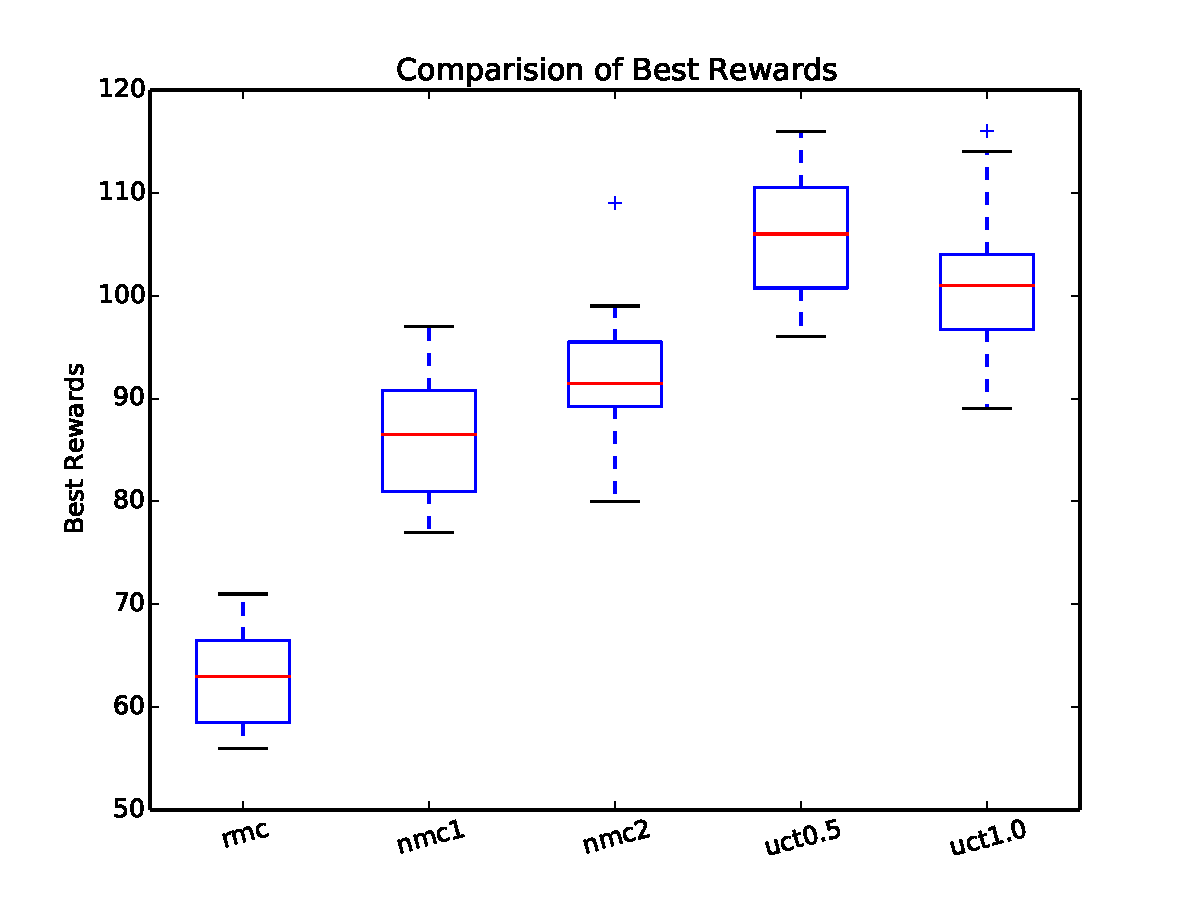
\includegraphics[width=0.8\textwidth]{best_reward_compare.pdf}
\caption{\label{fig:optimality}Comparision of Best Rewards}
\end{figure}

\begin{figure}[htbp!]
\centering
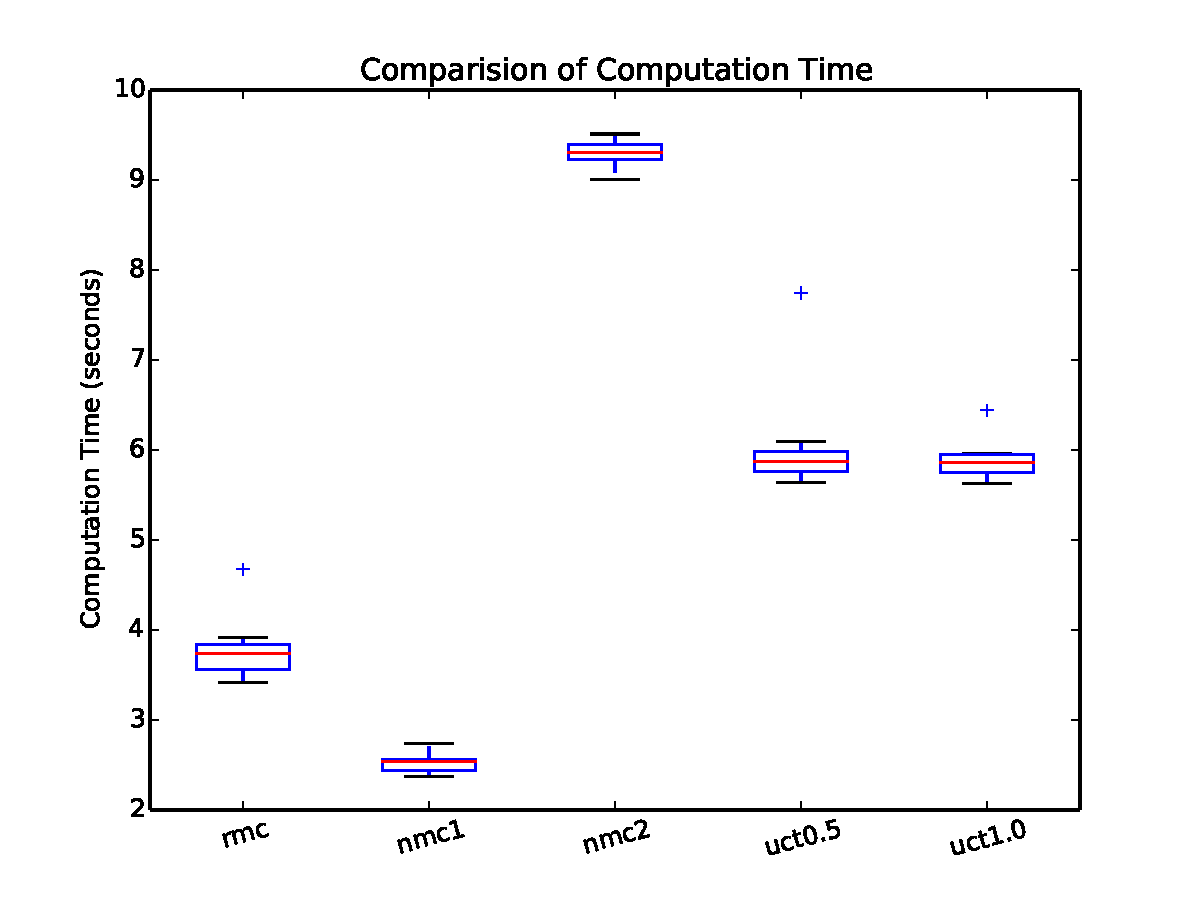
\includegraphics[width=0.8\textwidth]{computation_time_compare.pdf}
\caption{\label{fig:computation_time}Comparision of Computation Time}
\end{figure}

\begin{figure}[htb!]
\centering
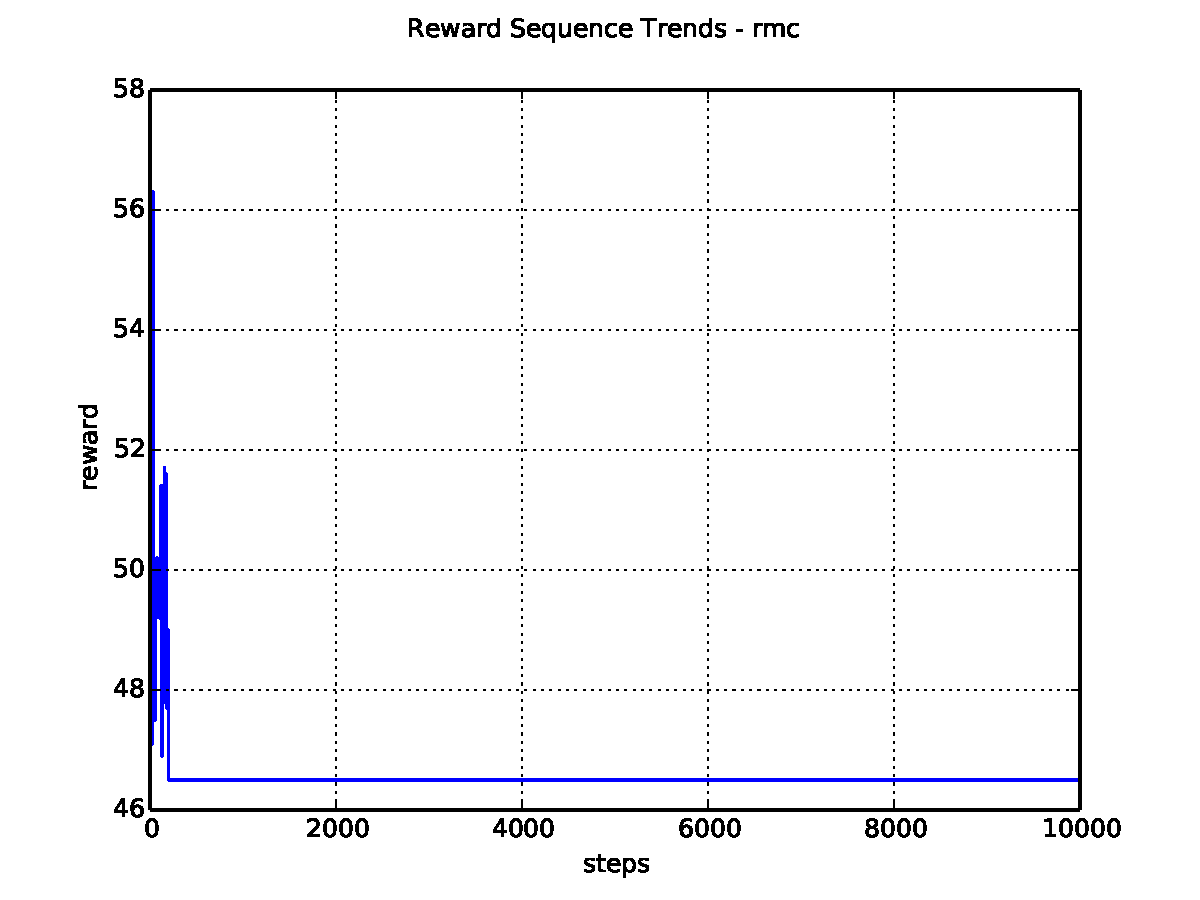
\includegraphics[width=0.8\textwidth]{trends_rmc.pdf}
\caption{\label{fig:trends_rmc}Trends of Reward Sequence for rmc}
\end{figure}

\begin{figure}[htb!]
\centering
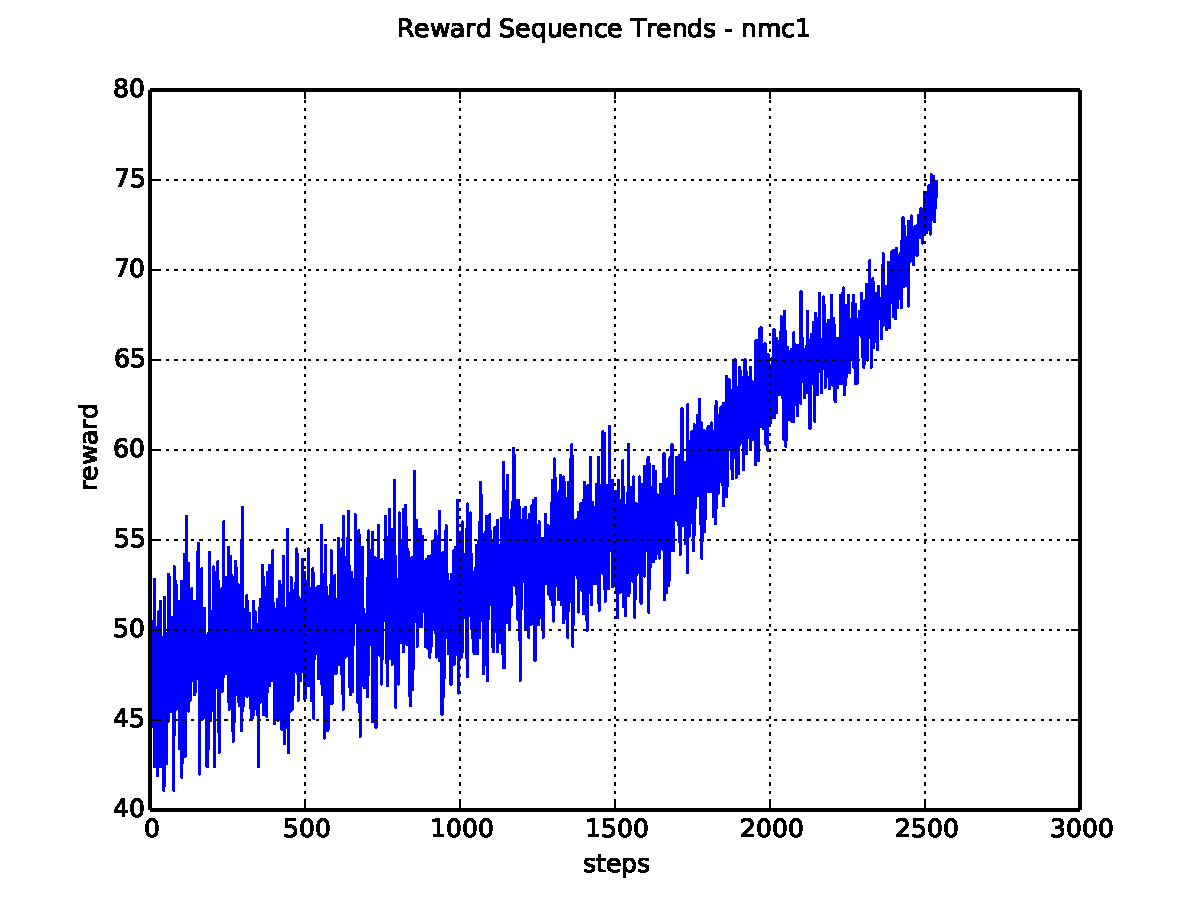
\includegraphics[width=0.8\textwidth]{trends_nmc1.pdf}
\caption{\label{fig:trends_nmc1}Trends of Reward Sequence for nmc1}
\end{figure}

\begin{figure}[htb!]
\centering
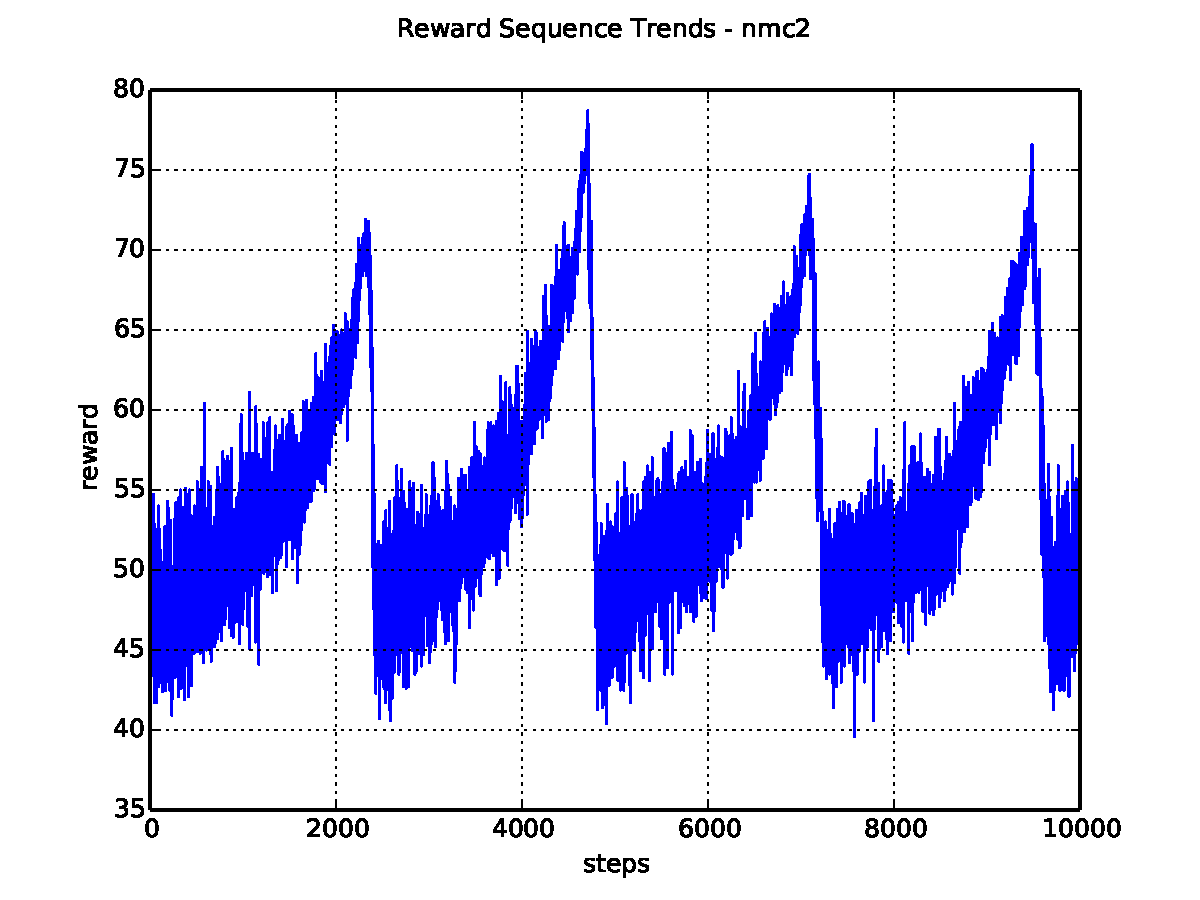
\includegraphics[width=0.8\textwidth]{trends_nmc2.pdf}
\caption{\label{fig:trends_nmc2}Trends of Reward Sequence for nmc2}
\end{figure}

\begin{figure}[htb!]
\centering
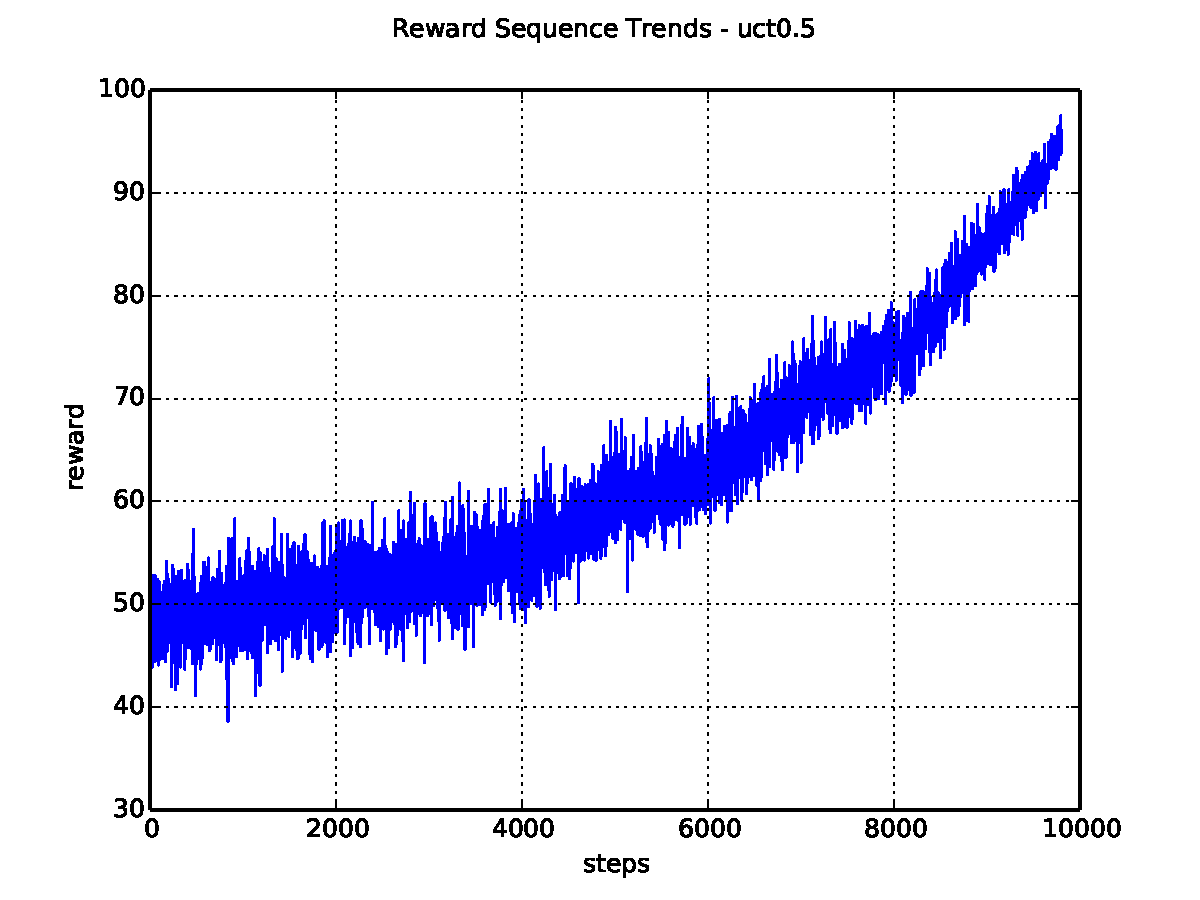
\includegraphics[width=0.8\textwidth]{trends_uct0_5.pdf}
\caption{\label{fig:trends_uct0.5}Trends of Reward Sequence for uct0.5}
\end{figure}

\begin{figure}[htb!]
\centering
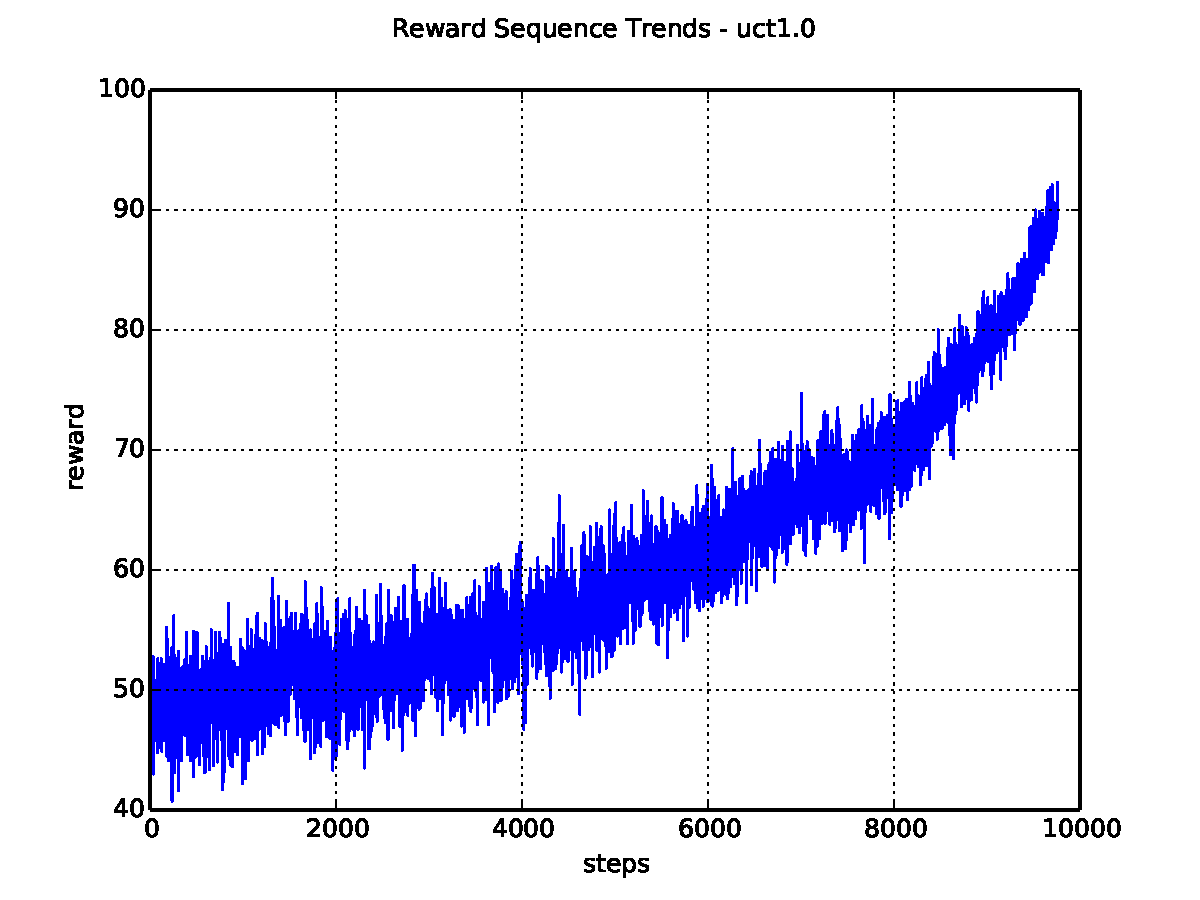
\includegraphics[width=0.8\textwidth]{trends_uct1_0.pdf}
\caption{\label{fig:trends_uct1.0}Trends of Reward Sequence for uct1.0}
\end{figure}



\subsection{Best Reward}
The current best rewards for each datasets are in Table \ref{tab:best_rewards}.

\begin{table}[htbp]
  \centering
  \caption{Illustration of search components}
    \begin{tabular}{cc}
    \toprule
    dataset & current best reward \\
    \midrule
    set 1 & 19 \\
    set 2 & 157 \\
    set 3 & 2612 \\
    set 4 & 248 \\
    set 5 & 1170 \\
    set 6 & 587 \\
    set 7 & 9979 \\
    \bottomrule
    \end{tabular}%
  \label{tab:best_rewards}%
\end{table}%xs

\section{Conclusion}
This study implemented the general framework of MCTS to solve the network population problem. Preliminary comparision of different algorithms demonstrates that uct0.5 and uct1.0 perform best in both criterias of best rewards detection and computation time, especially, uct seems like possessing the abality of learning. Future work may focus on the more detailed comparisions between different algorithms (eg. based on a meta multi-armed bandit problems). Also, a fast and efficient approach to detect new candidate nodes set and calculate the total reward of network should be explored. Most importantly, rather than treating select search component as a simple multi-armed bandit problem, more infomation should also be recored for the deeper nodes. Lastly, the better understanding of the network and original color sequence is indispensable. Due to time limitation, this work still needs more effort to improve the best reward and detect more efficient algorithm based on the general framework of MCTS. 

% References section
\nocite{*}
\bibliographystyle{unsrt}
\bibliography{main}
\addcontentsline{toc}{chapter}{References}

\newpage

\section*{Appendix A - Comparision of Algorithms}

\begin{table}[htbp]
  \centering
  \caption{Comparision of Best Rewards}
    \begin{tabular}{ccccccccccccc}
    \toprule
    algorithm &  run 1 & run 2 & run 3 & run 4 & run 5 & run 6 & run 7 & run 8 & run 9 & run 10 & mean & std\\
    \midrule
    rmc & 71 & 63 & 71 & 63 & 56 & 58 & 67 & 60 & 58 & 65 & 63.20 & 5.06\\
    nmc1 & 81 & 93 & 97 & 80 & 90 & 77 & 91 & 90 & 83 & 81 & 86.30 & 6.34 \\
    nmc2 & 99 & 94 & 89 & 96 & 80 & 84 & 92 & 109 & 91 & 90 & 92.30 & 7.61 \\
    uct0.5 & 109 & 114 & 111 & 100 & 100 & 103 & 116 & 103 & 109 & 96 & 106.10 & 6.30 \\
    uct1.0 & 104 & 89 & 114 & 100 & 116 & 102 & 96 & 99 & 94 & 104 & 101.80 & 7.93 \\
    \bottomrule
    \end{tabular}%
  \label{tab:best_rewards_compare}%
\end{table}%xs

\begin{table}[htbp!]
  \centering
  \caption{Comparision of Computation Time (seconds)}
    \begin{tabular}{ccccccccccccc}
    \toprule
    algorithm &  run 1 & run 2 & run 3 & run 4 & run 5 & run 6 & run 7 & run 8 & run 9 & run 10 & mean & std\\
    \midrule
    rmc & 4.675 & 3.800 & 3.553 & 3.413 & 3.568 & 3.671 & 3.840 & 3.820 & 3.915 & 3.354 & 3.78 & 0.33 \\
    nmc1 & 2.429 & 2.541 & 2.550 & 2.566 & 2.531 & 2.373 & 2.441 & 2.742 & 2.445 & 2.656 & 2.53 & 0.11 \\
    nmc2 & 9.260 & 9.407 & 9.511 & 9.202 & 9.009 & 9.344 & 9.255 & 9.366 & 9.435 & 9.214 & 9.30 & 0.14 \\
    uct0.5 & 5.746 & 5.793 & 7.746 & 5.644 & 5.916 & 6.091 & 5.679 & 5.927 & 5.823 & 6.000 & 6.04 & 0.59 \\
    uct1.0 & 5.873 & 5.833 & 5.952 & 5.626 & 5.929 & 5.662 & 5.859 & 6.441 & 5.727 & 5.965 & 5.89 & 0.22 \\
    \bottomrule
    \end{tabular}%
  \label{tab:computation_time_compare}%
\end{table}%xs

\section*{Appendix B - Source Code}
%\begin{lstlisting}[language={python}]
\begin{python}[moreemph={[4]42},caption={A General Framework of MCTS based on Python},label=ex1]
# -*- coding: utf-8 -*-
"""
Created on Wed Oct  8 12:45:20 2014

@author: liuweizhi
"""
import os,sys,glob
import random
import matplotlib.pyplot as plt
import networkx as nx
import numpy as np
import math
import copy
import shelve
import easygui

class GameTree():
    def __init__(self):
        self.graph = []
        self.sequence = []
        return 
    def initialization(self, graphdir, seqdir):
        ''' return the constructed graph and sequence '''
        ## build the network
        f_graph = open(graphdir, 'r')
        content = f_graph.read().replace('\n', ' ').strip(' ').split(' ')
        content = [int(foo) for foo in content]
        scale =  max(content) - min(content) + 1
        f_graph.close()
        ### initialize the adjacent network with scale * scale (graph[i,j] means the
        ### number of edges between node i and node j)
        graph = np.matrix([[ 0 for j in range(scale)] for i in range(scale)])
        f_graph = open(graphdir, 'r')        
        for line in f_graph:
            tmp = line.strip('\n').split(' ')
            try:
                [v1, v2] = [int(tmp[i]) - min(content) for i in range(len(tmp))]
                if (v1 != v2):
                    graph[v1,v2] = graph[v1,v2] + 1
                    graph[v2,v1] = graph[v2,v1] + 1
                else:
                    graph[v1,v2] = graph[v1,v2] + 1
            except:
                print "the sequence file isn't complete"
                sys.exit(0)
        self.graph = graph                 
        f_graph.close()
        ## record the sequence
        sequence = []
        f_seq = open(seqdir, 'r')
        content = f_seq.read().strip('\n')
        for color in content:
            color = int(color)
            if color == 0:
                sequence.append(-1)
            elif color == 1:
                sequence.append(1)
            else:
                print "the color sequence contains number other than 0 or 1!!!!"
                sys.exit(0)
        self.sequence = sequence
        f_seq.close()
        return [self.graph, self.sequence]
  
class MCTS():
    def __init__(self):
        self.name = 'Noname'
        self.best_population = []
        self.best_reward = -9999
        self.graph = []
        self.sequence = []
        self.setdir = ''
        return
        
    def initialization(self, graph, sequence, setdir):
        self.best_population = []
        self.best_reward = -9999
        self.graph = graph
        self.sequence = sequence
        # self.setdir is for the self.output() method
        self.setdir = setdir
        return 
    
    def step(self, population, candi, func_list):
        ''' given unifinished population, return the best population and best reward
        which are constructed step by step '''
        # generate the population step by step
        id = len(population) + 1
        while not(self.terminal(population, candi)):
            population = self.invoke(population, candi, func_list)
            # update the next candidate space
            candi = self.candidate(population[0:id-1], [population[id-1]], candi)
            # only obtain the id th element from the population derived from
            # self.invoke, step by step
            population = population[0:id]
            id = id + 1
        # update the best_population and best_reward
        self.evaluate(population)
        return population
        
    def repeat(self, population, candi, func_list, N):
        ''' repeat n simulations using given search component and return the best
        population sequence '''
        best_population = []
        best_reward = -9999
        for i in range(N):
            tmp_population = self.invoke(population, candi, func_list)
            tmp_reward = self.reward(tmp_population)
            if tmp_reward > best_reward:
                best_population = tmp_population
                best_reward = tmp_reward
        return best_population
    
    def lookahead(self, population, candi, func_list):
        ''' return the all possible population for the next step '''
        best_population = []
        best_reward = -9999
        for new_node in candi:
            # generate the new_population by append the new node to original population
            new_candi = self.candidate(population, [new_node], candi)
            new_population = [foo for foo in population]            
            # just lookahead 
            new_population.append(new_node)
            # further generate a new population sequence given new_population
            tmp_population = self.invoke(new_population, new_candi, func_list)
            tmp_reward = self.reward(tmp_population)
            # update the best_population and best_reward
            if tmp_reward > best_reward:
                best_population = tmp_population
                best_reward = tmp_reward
        return best_population
        
    def select(self, population, candi, N, thr, func_list):
        ''' given population, then select the next population state using UCB with
        explorer parameter thr and budget N * len(candi)'''        
        best_population = []
        best_reward = -9999
        # initialize the reawrd and number of trials of the total len(candir) arms
        arms = [{'reward':0, 'trial':0} for i in range(len(candi))]
        ucb = [0 for i in range(len(arms))]
        total_trials = 0
        untried = [foo for foo in candi]
        # the total budget is N
        candi_budget = len(candi)
        population_budget = int((1 - (self.graph.shape[0] * float(N)) / len(candi)) *
              (len(population) / float(len(self.sequence))) +  (self.graph.shape[0] *
               float(N)) / len(candi))
        for i in range(candi_budget * population_budget):
            # exists some untried arms
            if untried:
                new_node = untried[int(random.uniform(0,len(untried)))]
                untried.remove(new_node)
            # all arms were tried, then using the ucb value to select next state
            else:
                new_node = candi[ucb.index(max(ucb))]
            # generate the next population
            sub_candi = self.candidate(population, [new_node], candi)
            sub_population = [foo for foo in population]
            sub_population.append(new_node)
            tmp_population = self.invoke(sub_population, sub_candi, func_list)
            tmp_reward = self.reward(tmp_population)
            # update best_population and best_reward
            if tmp_reward > best_reward:
                best_population = tmp_population
                best_reward = tmp_reward
            # update the attributes of arms and calculate the ucb value
            arm_id = candi.index(new_node)
            arms[arm_id]['reward'] += tmp_reward
            arms[arm_id]['trial'] += 1.0
            total_trials += 1.0
            #reward_ucb = arms[arm_id]['reward'] / (algo.best_reward * arms[arm_id]['trial'])
            #trial_ucb = 1.0 / (1.0 + math.exp(- math.sqrt(2 * math.log(total_trials)
                        # / arms[arm_id]['trial'])))
            reward_ucb = arms[arm_id]['reward'] / arms[arm_id]['trial']
            trial_ucb = math.sqrt(2 * math.log(total_trials) / arms[arm_id]['trial'])
            ucb[arm_id] = reward_ucb + thr * trial_ucb
        return best_population
        
    def simulate(self, population, candi):
        ''' return a randomly population sequence given current unfinished population
        sequence '''      
        graph = self.graph 
#        # states_seq is empty which means the initial state of simulation
#        if [] == population:
#            new_node = candi[int(random.uniform(0,len(candi)))]
#            population.append(new_node)
        # generate the uniformly randomly simulation population sequence
        while(not(self.terminal(population, candi))):
            new_node = candi[int(random.uniform(0, len(candi)))]
            candi = self.candidate(population, [new_node], candi)
            population.append(new_node)
        self.evaluate(population)       
        return population

    def candidate(self, population, new_node, candi):
        ''' return the next candidate space given the population '''
        # return the ajcacent vector of new_node
        if (population==[]) and (new_node==[]) and (candi==[]):
            candi = list(np.where(self.graph.sum(axis=0).A1>0)[0])
        elif (population==[]) and (new_node) and (candi):
            new_node_neighbor = []
            for foo in new_node:
                new_node_neighbor.extend(np.where(self.graph[foo,].A1>0)[0].tolist())
            candi = list(set(new_node_neighbor) - set(new_node))
        else:
            new_node_neighbor = []
            for foo in new_node:
                new_node_neighbor.extend(np.where(self.graph[foo,].A1>0)[0].tolist())
            try:
                candi = list((set(candi) | set(new_node_neighbor)) - set(new_node)
                        - set(population))
            except:
                print 'candi',candi
                print 'new_node_neighbor',new_node_neighbor
                print 'new_node',new_node
                print 'population',population
                sys.exit(0)
        return candi
        
    def evaluate(self, population):
        ''' return the best_population, best_reward of the upper search component
        and the population evaluated, and check if the budget is run out '''
        global numCalls
        global budget
        # calculate the reward given finished population sequence
        reward = self.reward(population)
        # update the best_reward and best_population
        if reward > self.best_reward:
            self.best_reward = reward
            self.best_population = [population]  
        elif reward == self.best_reward:
            self.best_population.append(population)
        # update the budget usage
        numCalls = numCalls + 1
        print '%s - (%d/%s) - best reward: %d/%d' % (self.name, numCalls, str(budget),
               self.best_reward, reward)
        if numCalls == budget:
            print 'the budget has been run out'
            # output the current best population and reward
            # self.output(self.best_population[0], self.best_reward)
            sys.exit(0) # need modify
        return reward
    
    def invoke(self, population, candi, func_list):
        if not(self.terminal(population, candi)):
            func = func_list[0]
            population = func['func'](population, candi, **func['argv'])
        else:
            self.evaluate(population)
        return population
    
    def reward(self, population):
        ''' return the reward of the graph given population sequence'''
        graph = self.graph
        sequence = self.sequence
        # for color_seq, if the value == 0, then it means the corresponding node isn't
        # painted
        color_seq = np.matrix([0 for v in range(self.graph.shape[0])])
        for v in population:
            color_seq[0, v] = sequence[population.index(v)]
        return int(np.square(color_seq) * graph * np.square(color_seq).T - color_seq * graph * color_seq.T) / 4
        
    def terminal(self, population, candi):
        ''' return whether entering the terminal state '''
        if (population):
            if (candi and (len(population)<len(self.sequence))):
                flag = False
            else:
                flag = True
        # the initial state of population
        else:
            flag = False
        return flag
        

    def output(self, population, reward):
        ''' write the reward and population sequence into txt files '''
        # write reward into file    
        checker = ['Lim Wei Quan', 'Lim Wei Zhong', 'Zhang Chen']
        f_reward = open(os.path.join(self.setdir, 'reward.txt'), 'w')
        f_reward.write('reward=%d\n' % reward)
        for foo in checker:
            f_reward.write('%s\n' % foo)
        f_reward.close()
        # write population sequence and corresponding color sequence into file
        sequence = self.sequence
        f_population = open(os.path.join(self.setdir, 'population.txt'), 'w')
        for i in range(len(population)):
            f_population.write('%d %d\n' % (population[i], (self.sequence[i]+1)/2))
        f_population.close()
        return 
    
    
def recursive(func_list):
    ''' return the self-loop recursive func_list given func_list '''
    for i in range(len(func_list)-1):
        func_list[i]['argv']['func_list'] = func_list[i+1:len(func_list)]
    return func_list  
 
def combinator(func_list):
    ''' run the recurisive func '''
    func_list = recursive(func_list)
    func = func_list[0]
    result = func['func'](**func['argv'])
    return result
    
def restore_shelve(filename):
    ''' restore the workspace '''
    f_shelf = shelve.open(filename)
    for key in f_shelf:
        globals()[key] = f_shelf[key]
    f_shelf.close()
    return 
### parameters initialization
random.seed(5330)
### read file    
homedir = os.getcwd()
datadir = os.path.join(homedir, 'data/submission')
datalist = os.listdir(datadir)
for foo in datalist:
    # initialize the game tree
    if 'set' in foo:
        setdir = os.path.join(datadir, foo)
    else:
        continue
    graphdir = glob.glob('%s/graph*.txt' % setdir)[0]
    seqdir = glob.glob('%s/seq*.txt' % setdir)[0]
    tree = GameTree()
    [graph, sequence] = tree.initialization(graphdir, seqdir)

    # create MCTS() class algo to let the algo_list legal
    algo = MCTS()
    algo.initialization(graph, sequence, setdir)
    population = []
    candi = algo.candidate([], [], [])
    # specify the algorithms we want to use like UCT, Nested Monte Carlo Tree
    algo_list = {
       'rmc': [{'func':algo.step, 'argv':{'population':population, 'candi':candi}},
               {'func':algo.repeat, 'argv':{'N':10000}}, {'func':algo.step, 'argv':{}},
               {'func':algo.repeat, 'argv':{'N':10}}, {'func':algo.simulate, 'argv':{}}],
       'nmc1': [{'func':algo.step, 'argv':{'population':population, 'candi':candi}},
                {'func':algo.lookahead, 'argv':{}}, {'func':algo.simulate, 'argv':{}}],
       'r-nmc1': [{'func':algo.repeat, 'argv':{'population':population, 'candi':candi, 'N':100}},
                  {'func':algo.step, 'argv':{}}, {'func':algo.lookahead, 'argv':{}},
                  {'func':algo.simulate, 'argv':{}}],                
       'nmc2': [{'func':algo.step, 'argv':{'population':population, 'candi':candi}},
                {'func':algo.lookahead, 'argv':{}}, {'func':algo.step, 'argv':{}},
                {'func':algo.lookahead, 'argv':{}}, {'func':algo.simulate, 'argv':{}}],
        # uct algorithms computation time : len(seq) * N_repeat * (N_graph * len(graph)
        # + 1) * len(seq) / 2
       'uct0.5': [{'func':algo.step, 'argv':{'population':population, 'candi':candi}},
                  {'func':algo.repeat, 'argv':{'N':1}},
                  {'func':algo.select, 'argv':{'N': 2, 'thr':0.5}},
                  {'func':algo.simulate, 'argv':{}}],
       'uct1.0': [{'func':algo.step, 'argv':{'population':population, 'candi':candi}},
                  {'func':algo.repeat, 'argv':{'N':1}},
                  {'func':algo.select, 'argv':{'N': 3, 'thr':1.0}},
                  {'func':algo.simulate, 'argv':{}}],                 
       'r1': [{'func':algo.select, 'argv':{'population':population, 'candi':candi, 'N':100, 'thr':0.5}},
              {'func':algo.step, 'argv':{}}, {'func':algo.repeat, 'argv':{'N':100}},
              {'func':algo.select, 'argv':{'N':1000, 'thr':0.5}},
              {'func':algo.simulate, 'argv':{}}],
    }
    
    # the candidate algorithms to be compared
    algo_candi = ['uct0.5', 'rmc', 'nmc1']
    best_population = []
    best_reward = -9999
    algo_result = []
    for foo in algo_candi:
        # define the basic parameter
        global budget
        budget = float('inf')
        global numCalls
        numCalls = 0        
        # initial the algo (clear the previous algorithm's best_population and
        # best_reward in algo)
        algo.initialization(graph, sequence, setdir)
        algo.name = foo
        # run the algorithms based on the foo
        combinator(algo_list[foo])
        reward = algo.reward(algo.best_population[0])
        # update the best population and best reward
        if reward > best_reward:
            best_population = [foo for foo in algo.best_population[0]]
            best_reward = reward
        # record the result of algo based on foo
        algo_result.append(copy.deepcopy(algo))
    # output the global best population, best reward given the comparision of all
    # algorithms in algo_candi
    algo.output(best_population, best_reward)
    # save the current workspace 
    f_shelf = shelve.open(os.path.join(setdir, 'workspace.out'), 'n')
    for key in dir():
        try:
            f_shelf[key] = globals()[key]
        except:
            print 'ERROR shelving: {0}'.format(key)
    f_shelf.close()
    
    # notify the programmer that the simulation is done
    print '\a'*7
    #easygui.msgbox("Simulation is Done", title="Message")
\end{python}
%\end{lstlisting}

\end{document}
